\documentclass[]{scrreprt}
\usepackage[spanish]{babel}
\usepackage[utf8]{inputenc}
\usepackage{listings}
\usepackage{underscore}
\usepackage{multirow}
\usepackage[table,xcdraw]{xcolor}
\usepackage{adjustbox}
\usepackage{graphicx}
\usepackage{float}
\usepackage[bookmarks=true]{hyperref}
\hypersetup{
    bookmarks=false,    % show bookmarks bar?
    pdftitle={Pruebas de sistema y de aceptación},    % title
    pdfauthor={Ivan Szkrabko},                     % author
    pdfsubject={TeX and LaTeX},                        % subject of the document
    pdfkeywords={TeX, LaTeX}, % list of keywords
    colorlinks=true,       % false: boxed links; true: colored links
    linkcolor=blue,       % color of internal links
    citecolor=black,       % color of links to bibliography
    filecolor=black,        % color of file links
    urlcolor=purple,        % color of external links
    linktoc=page            % only page is linked
}
\def\myversion{2.0}
\title{
\flushleft
\Huge{Pruebas de sistema y de aceptación}\\
\vspace{1cm}
para\\
\vspace{1cm}
Realidad aumentada para la optimización de procedimientos batch en la industria\\
\vspace{1cm}
\LARGE{Versión 1.0\\}
\vspace{1cm}
Realizado por Iván Szkrabko\\
}
\begin{document}
\maketitle
\tableofcontents
\chapter{Introducción}
El propósito de este sistema es innovar en la interacción entre los operadores y los sistema de
control distribuidos, para impulsar nuevas soluciones en el área de la automatización industrial.
Se busca explorar las oportunidades que ofrece la realidad aumentada para mejorar y optimizar
las tareas de los operadores, además de agilizar el entrenamiento de nuevos operarios y mejorar
la seguridad para procedimientos bajo situaciones de emergencia.

\chapter{Pruebas del sistema}
Las pruebas de sistema aseguran el cumplimiento de los requerimientos del proyecto. El sistema puede ser dividido en los siguientes subsistemas:


\begin{itemize}
	\item Interfaz usuario
	\item Servidor Local
	\item Cliente OPC
	\item Sistema control
\end{itemize}

Para el análisis se aplicara el Classification-Tree Method al subsistema denominado: Cliente OPC.

\section{Requerimientos}

Los requerimientos del mismo son:
\begin{itemize}
	\item El subsistema deberá ser capaz de subscribirse a un conjunto de variables OPC.
	\item El subsistema deberá alertar en caso de una falla de comunicación.
	\item El subsistema deberá alertar en caso de una mala calidad de datos.
	\item El subsistema deberá ser capaz de escribir en una ruta OPC determinada.
	\item El subsistema deberá ser capaz de leer en una ruta OPC determinada.
\end{itemize}

\section{Aspectos del objeto de prueba}

\begin{itemize}
	\item Suscripción lectura
	\item Falla de comunicación.
	\item Mala calidad de datos.
	\item Escritura de datos
	\item Lectura de datos
\end{itemize}
	
\section{Casos de prueba lógicos}

\begin{figure}[H]
  \centering
  \vspace{1cm} 
  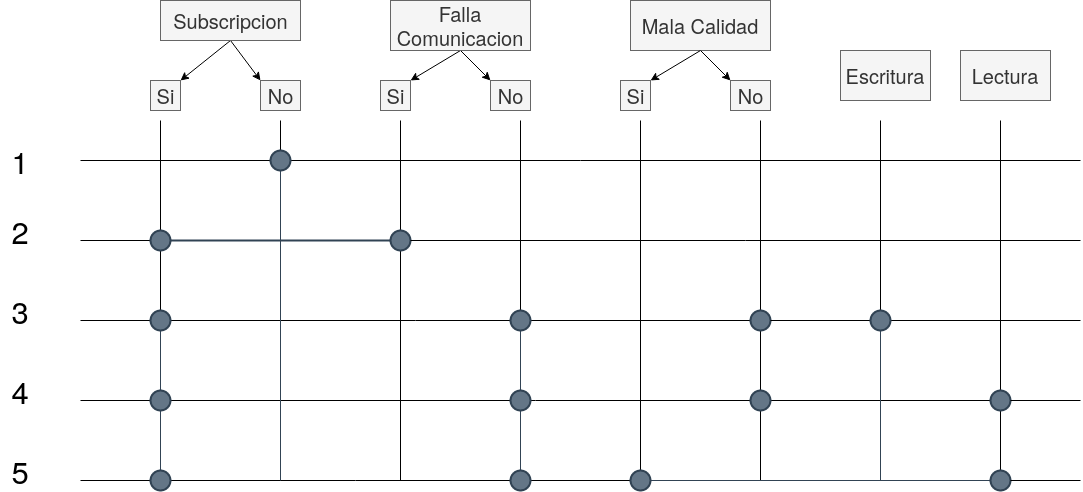
\includegraphics[width=1.15\textwidth]{CTM.png}
  \vspace{1cm} 
\end{figure}

\section{Definición de los casos de prueba}

Caso: 1
\begin{itemize}
	\item Valores de entrada: la suscripción no se ha efectuado
	\item Resultados esperados: el sistema no debe tener conocimiento de la variable 
\end{itemize}

Caso: 2
\begin{itemize}
	\item Valores de entrada: la variable fue suscrita pero hay una falla de comunicación.
	\item Resultados esperados: el sistema debe alertar de la falla critica.
\end{itemize}

Caso: 3
\begin{itemize}
	\item Valores de entrada: la variable fue suscrita y hay buena calidad de datos, se ejecuta el comando de escritura.
	\item Resultados esperados: el sistema debe actualizar el estado de la variable opc en el servidor.
\end{itemize}

Caso: 4
\begin{itemize}
	\item Valores de entrada: la variable fue suscrita y hay buena calidad de datos, se ejecuta el comando de lectura.
	\item Resultados esperados: el sistema debe leer el estado de la variable del servidor y reportarla en la interfaz visual del operador.
\end{itemize}

Caso: 5
\begin{itemize}
	\item Valores de entrada: la variable fue suscrita pero no hay buena calidad de datos, se ejecuta el comando de lectura.
	\item Resultados esperados: el sistema debe alertar de la mala calidad de datos al operador, con un tag (BQ) indicando "Bad Quality". 
\end{itemize}

\end{document}
